% siminos/atlas/cut.tex  pdflatex atlas
% $Author$ $Date$

\section{Sections}
\label{s:cut}

In the {\em Poincar\'e section} method one records the coordinates of the
trajectory $\ssp(\zeit)$ at the instant $\sspRed_n = \ssp(\zeit_n)$
it traverses the fixed oriented hypersurface $\PoincS$ of
codimension 1. For high-dimensional flows that we have in mind, the
practical choice is a hyperplane, the type of Poincar\'e section (or,
from now on, just a \emph{section})  we shall consider here. Such a
section captures important features of the flow in an open neighborhood
of the section-fixing \template.

%%%%%%%%%%%%%%%%%%%%%%%%%%%%%%%%%%%%%%%%%%%%%%%%%%%%%%%%%%%%%%%%%%%%%
\begin{figure}
  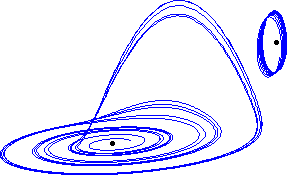
\includegraphics[width=0.3\textwidth]{RoessTrjs}
    \caption{
R\"ossler \eqva\ and their invariant manifolds. The stable manifold of
the inner {\eqv} $\ssp_{-}$  is 1-dimensional and the unstable one is a
spiral-out focus. For the outer {\eqv} $\ssp_{+}$  the stable manifold is
a spiral-in focus (basin boundary for initial conditions that either fall
into the chaotic attractor, or escape to infinity) and the unstable
manifold is 1-dimensional.
    }
\label{fig:RoessTrjs}
\end{figure}
%%%%%%%%%%%%%%%%%%%%%%%%%%%%%%%%%%%%%%%%%%%%%%%%%%%%%%%%%%%%%%%%%%%%%

As an example consider the system of R\"ossler\rf{ross},
\index{R\"ossler system}
\beq
\begin{split}
  \dot{x} &= -y \,-\,z \\
  \dot{y} &= x + a y \\
  \dot{z} &= b + z (x - c)
  \,,
  \label{eq:Rossler}
\end{split}
\eeq
where $a = b = 0.2$ and $c = 5.7$. This flow has two prominent invariant
states, the `inner' $\ssp_{-}$ and the `outer' $\ssp_{+}$ unstable \eqva\
(\refFig{fig:RoessTrjs}) which we pick as {\em \template s}.

We orient the sections so the plane $\PoincS_{-}$ contains the 1\dmn\
stable eigenvector (\reffig{fig:RoessNearEq}), and the other section
$\PoincS_{+}$ contains the 1\dmn\ unstable eigenvector
(\reffig{fig:RoessFarEq}), thus capturing the local spiral-in,
spiral-out dynamics. The remaining freedom to rotate each section can be
used to orient them in such a fashion that the ridge (the intersection of
the two sections) lies approximately midways between the two templates
(\reffig{fig:RoessBothEq}).
    \DB{2012-04-10}{
    Not really sure how this last bit fits into this part at this time.
    It is unclear why we are doing this. I would consider moving this to
    discussion of 2-chart atlas. 2012-04-10 Predrag: is the text better
    now?
    }

A well chosen section captures the dynamics in the neighborhood of its
\template, but how far does this neighborhood extend?
The answer is that the section captures neighboring trajectories as long
as it cuts them transversally; it fails the moment the velocity field at
point $\sspRSing$ fails to pierce the section. At these locations, the
velocity either vanishes (\eqv) or is tangent to the section, \ie,
orthogonal to the section normal $\hat{n}$,
\beq
    \hat{n} \cdot \vel(\sspRSing) = 0
\,,\qquad
    \sspRSing \in \cal{S}
\,.
\ee{eq:sspRSing}
For a smooth flow such points form a smooth $(d\!-\!2)$\dmn\
\emph{\poincBord} ${\cal S} \subset \PoincS$ encompassing the open
neighborhood of the {\template} characterized by qualitatively similar
flow, and beyond which the flow pierces the section hyperplane in the `wrong'
direction. We shall refer to such region of a section hyperplane as a
`chart' of the {\template} neighborhood.


%%%%%%%%%%%%%%%%%%%%%%%%%%%%%%%%%%%%%%%%%%%%%%%%%%%%%%%%%%%%%%%%%%%%%
\begin{figure}%[H]
\begin{center}
  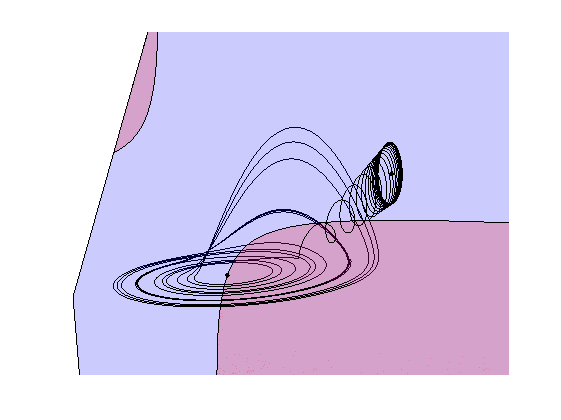
\includegraphics[width=0.30\textwidth,clip=true]{RoessNearEq}
\end{center}
  \caption{\label{fig:RoessNearEq}
  A R\"ossler flow Poincar\'e section $\PoincS_{-}$ through the inner
  {\eqv} $\ssp_{-}$ and its stable eigenvector.
}
\end{figure}
%%%%%%%%%%%%%%%%%%%%%%%%%%%%%%%%%%%%%%%%%%%%%%%%%%%%%%%%%%%%%%%%%%%%%

%%%%%%%%%%%%%%%%%%%%%%%%%%%%%%%%%%%%%%%%%%%%%%%%%%%%%%%%%%%%%%%%%%%%%
\begin{figure}%[H]
\begin{center}
  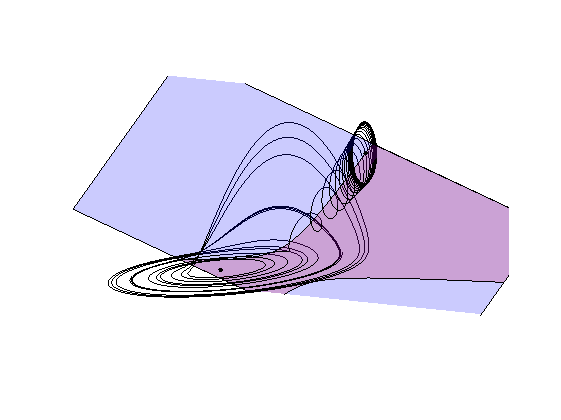
\includegraphics[width=0.30\textwidth,clip=true]{RoessFarEq}
\end{center}
  \caption[R\"ossler section, outer {\eqv}]{
  A Poincar\'e section for R\"ossler flow
      through the
      outer
  {\eqv} $\ssp_{+}$  and its unstable eigenvector.
  } \label{fig:RoessFarEq}
\end{figure}
%%%%%%%%%%%%%%%%%%%%%%%%%%%%%%%%%%%%%%%%%%%%%%%%%%%%%%%%%%%%%%%%%%%%%

%%%%%%%%%%%%%%%%%%%%%%%%%%%%%%%%%%%%%%%%%%%%%%%%%%%%%%%%%%%%%%%%%%%%%
\begin{figure}%[H]
\begin{center}
  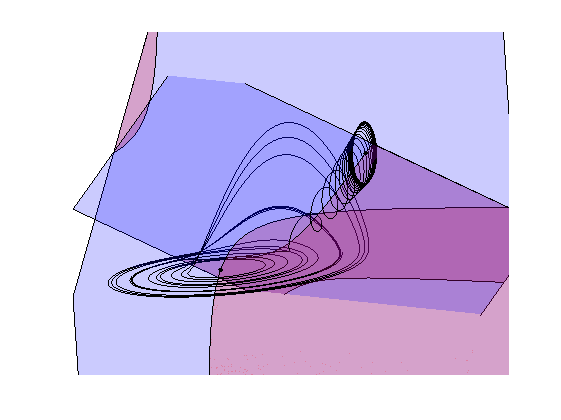
\includegraphics[width=0.30\textwidth,clip=true]{RoessBothEq}
\end{center}
  \caption{
  A two-section atlas for R\"ossler flow, with the local sections of
  \reffigs{fig:RoessNearEq}{fig:RoessFarEq} oriented and combined so that
  the ridge (intersection of the two sections, indicated by the brown
  line in individual sections) lies  approximately midway between the
  \template s.
  } \label{fig:RoessBothEq}
\end{figure}
%%%%%%%%%%%%%%%%%%%%%%%%%%%%%%%%%%%%%%%%%%%%%%%%%%%%%%%%%%%%%%%%%%%%%

%\subsection{R\"ossler two-chart atlas}

For R\"ossler flow \refeq{eq:Rossler} the \refeq{eq:sspRSing} is a
quadratic condition in 3 dimensions, so \poincBord\ is a conic section
drawn in the charts \reffigs{fig:RoessNearEq}{fig:RoessFarEq}. The two
charts meet in a ridge, and together do a pretty good job as the 2-chart
atlas of the interesting R\"ossler dynamics, \reffig{fig:RoessBothEq}. As
explained in ChaosBook.org, due to extreme contraction rate, the section
in \reffig{fig:RoessNearEq} is for all practical purposes 1\dmn, and the
associated return map yields all \po s of the 3\dmn\

In 3 dimensions everything -sections, ridges, \poincBord s-  can be
drawn. But what about high-dimensional flows? The point is that while it
is impossible to visualize  $(d\!-\!2)$\dmn\ {\poincBord}, a point is a
point, and a line is a line in a projection from any number of
dimensions, so a trajectory crossing of both a section and a {\poincBord}
can be easily determined and visualized in any dimension.

% \subsection{$N$-chart atlas, forward maps}
% \subsection{Ring of Fire return map\rf{lanCvit07}}

To summarize: we can chart a region of \statesp\ of interest, by a
picking a sufficient number of \template s and the associated charts,
each bounded by \poincBord s and ridges.

Two concluding remarks on what sections \emph{are not}:

(1) A Poincar\'e section is {\em not} a projection onto a
lower-dimensional space: Rather, it is a local change of coordinates to a
direction along the flow, and the remaining coordinates transverse to it.
No information about the flow is lost; the full space trajectory can
always be reconstructed by integration from a point in the section.

(2) The method of Poincar\'e sections is {\em not} equivalent to
\emph{strobing} a flow at a sequence of instants in time. While
`strobing' is what any numerical integrator does, by representing a
trajectory by a sequence of time-integration step separated points,
strobing is in general not a reduction of a flow to a codimension 1
manifold, as the sequence of strobed points still resides in the full
\statesp\ $\pS$, of dimensionality $d$.
